\newpage
\section{改良型細径羽状筋の開発}
%%%%%%%%%%%%%%%%%%%%%%%%%%%%%%%%%%%%%%%%%%%%%%%%%%%%%%%%%
\subsection{先行研究で確認された課題}
\subsection{課題1:細径MPAの制作方法の改良}
先行研究の細径MPA締結方法を図\ref{fig:MPA_tanbu_1}に示す.先行研究では,細径MPAを構成するシリコンチューブとスリーブを端部で糸で縛り接着剤で固定する方式を採用していた.
しかし,この方法では作製するのに時間がかかり,完成するのに技術が必要になってしまう.
そこで本研究では,\ref{fig:MPA_tanbu_2}のように細径MPA端部部品とOリングを用いた新しい細径MPA作製方法を開発した.
新型細径MPAの作製手順を以下に示す.従来の細径MPA作製方法を用いると作製時間が約20分なのに対し,本研究の作製方法では失敗することなく約10分で作製することができる.
\vspace{3mm}
\begin{enumerate}
  \item 図\ref{fig:MPA_tanbu_2_2}のようにゴムチューブを端部部品の溝部分に差し込み,差し込んだ隙間に接着剤を塗布する.反対側でも行う
  \item 接着剤が乾いたら,図\ref{fig:MPA_tanbu_2_1}のようにゴムチューブと端部部品をスリーブで包む
  \item 図\ref{fig:MPA_tanbu_2_1}のように図\ref{fig:MPA_tanbu_2_2}中のOリング固定溝にはまるようにOリングを配置する.反対側でも行う
  \item 端部部品,スリーブとOリングを固定するために接着剤を塗布する.反対側でも行う
\end{enumerate}
%%%%%%%%%%%%%%%%%%%%%%%%%%%%%%%%%%%%%%%%%%%%%%%%%%%%%%%%%
\begin{figure}[!hb]
  %
  \begin{minipage}{0.49\hsize}
    \centering  
    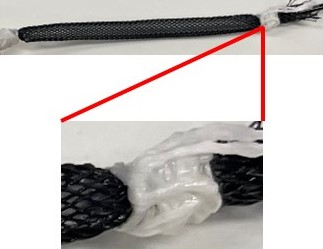
\includegraphics[scale=0.5]{image/MPA_tanbu_1_1.jpg}
    \subcaption{旧型細径MPA外観}
    \label{fig:MPA_tanbu_1_1}
  \end{minipage}
  %
  \begin{minipage}{0.5\hsize}
    \centering
    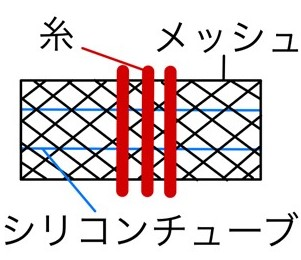
\includegraphics[scale=0.5]{image/MPA_tanbu_1_2.jpg}
    \subcaption{旧型細径MPA模式図}
    \label{fig:MPA_tanbu_1_2}
  \end{minipage}
  %
  \caption{先行研究で用いられた旧型細径MPA}
  \label{fig:MPA_tanbu_1}
\end{figure}
%
\begin{figure}[!hb]
  \begin{minipage}{0.49\hsize}
    \centering
    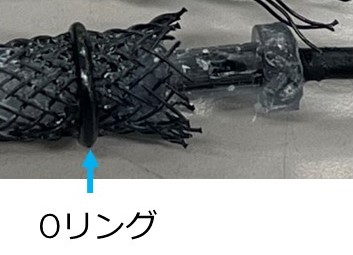
\includegraphics[scale=0.5]{image/MPA_tanbu_2_2.jpg}
    \subcaption{新型細径MPA外観}
    \label{fig:MPA_tanbu_2_1}
  \end{minipage}
  %
  \begin{minipage}{0.49\hsize}
    \centering  
    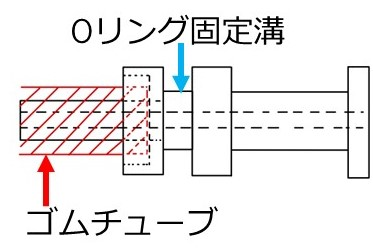
\includegraphics[scale=0.5]{image/MPA_tanbu_2_1.jpg}
    \subcaption{新型細径MPA模式図}
    \label{fig:MPA_tanbu_2_2}
  \end{minipage}
  \caption{本研究で用いた新型細径MPA}
  \label{fig:MPA_tanbu_2}
\end{figure}
%%%%%%%%%%%%%%%%%%%%%%%%%%%%%%%%%%%%%%%%%%%%%%%%%%%%%%%%%
\subsection{課題2:細径MPAの収縮率向上}
市販に売られている編組チューブは,図\ref{fig:messhu_henka}\subref{fig:messhu_1}のように断面が平たく折癖がついている.
その状態の編組チューブを用いて細径MPAを作成すると,図\ref{fig:MPA_henka}\subref{fig:MPA_1}のようにシリコンゴムチューブ(青色)と編組チューブの間に隙間が生じてしまう.
これにより,自身の径方向に膨張し軸方向に収縮する細径MPAにとっては収縮率が低下してしまう.
そこで本研究では,細径MPAの収縮性能を高めるために編組チューブを熱可塑変化させた.
大まかな作成方法をず\ref{fig:messhu_method}に示す.
図中\textcircled{\scriptsize 1}に示した物品が作製に必要なもので左から以下の通りである.
%
\begin{itemize}
  \item マスキングテープ テープ幅 15mm メーカー:モノタロウ 品番:15
  \item 編組チューブ 1×5(最小径×最大径) メーカー:モノタロウ 品番:-
  \item ステンレス丸棒 $\phi$ 2mm メーカー:モノタロウ 品番:1378
  \item ホットプレート メーカー:山善 品番:YHA-W102
\end{itemize}
%
熱可塑変化の手順を以下に示す.
\vspace{3mm}
\begin{enumerate}
  \item まず初めに,編み込みチューブをステンレス棒よりも 3cm程短い範囲で任意の長さに切る
  \item 編み込みチューブにステンレス棒を差し込む(図中\textcircled{\scriptsize 2})
  \item 編み込みチューブの内径がステンレス棒の外径になるようにマスキングテープで巻いて固定する(図中\textcircled{\scriptsize 3})
  \item ホットプレートを 180℃まで温めて,編み込みチューブ全体に熱が伝わるように転がしながら3分間温める(図中\textcircled{\scriptsize 4})
  \item 全体を冷水に漬けて,3分間ほど熱をとる(図中\textcircled{\scriptsize 5})
  \item 粗熱が取れたらマスキングテープを外して完成
\end{enumerate}
熱可塑変化させていない編組チューブを図\ref{fig:messhu_henka}\subref{fig:messhu_1},熱可塑変化させた編組チューブを図\ref{fig:messhu_henka}\subref{fig:messhu_2}に示す.
熱可塑変化させていない編組チューブは折癖あり,断面を平たいのに対し.熱可塑変化した編組チューブは折癖が取れ,断面を円形になっている.
この熱可塑変化させた編組チューブを用いて細径MPAを作製したものを図\ref{fig:MPA_henka}\subref{fig:MPA_2}に示す.
図\ref{fig:MPA_henka}\subref{fig:MPA_1}と比べるとシリコンチューブ(青色)と編組チューブの間が狭くなっていることがわかる.
熱可塑変化させたメッシュを用いて作製した新型細径MPAの収縮性能の変化を調べた.
熱可塑変化させていないメッシュを用いた旧型細径MPAの収縮率が 16%なのに対して,新型細径MPAの収縮率は 20%と向上したことを確認することができた.
%%%%%%%%%%%%%%%%%%%%%%%%%%%%%%%%%%%%%%%%%%%%%%%%%%%%%%%%%
%
\begin{figure}[ht]
  %
  \begin{minipage}{0.49\hsize}
    \centering  
    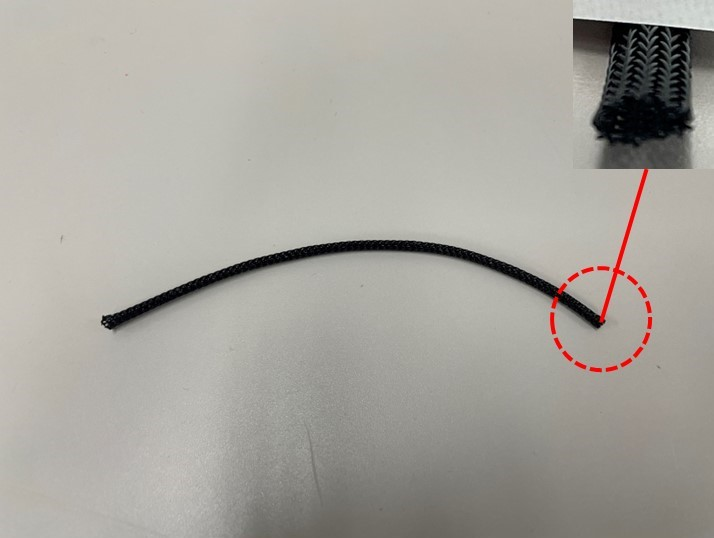
\includegraphics[scale=0.25]{image/messhu_hikaku_1.jpg}
    \subcaption{変化前}
    \label{fig:messhu_1}
  \end{minipage}
  %
  \begin{minipage}{0.49\hsize}
    \centering
    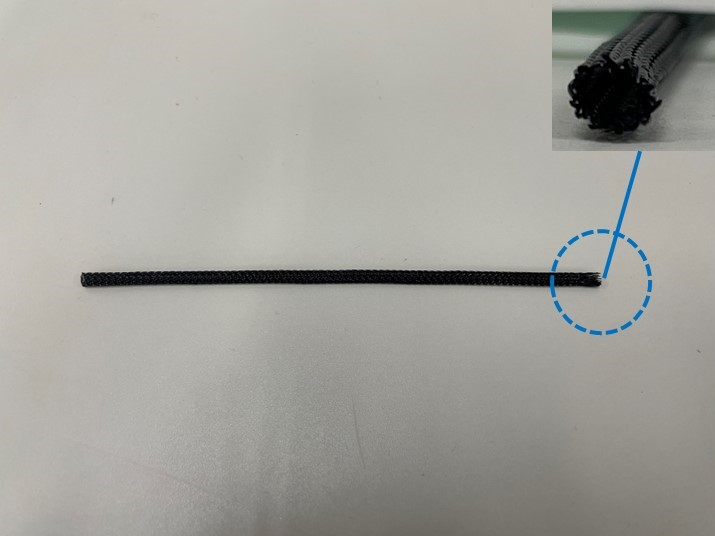
\includegraphics[scale=0.25]{image/messhu_hikaku_2.jpg}
    \subcaption{変化後}
    \label{fig:messhu_2}
  \end{minipage}
  %
  \caption{メッシュの熱可塑変化の様子}
  \label{fig:messhu_henka}
\end{figure}
%
\begin{figure}[ht]
  %
  \begin{minipage}{0.49\hsize}
    \centering  
    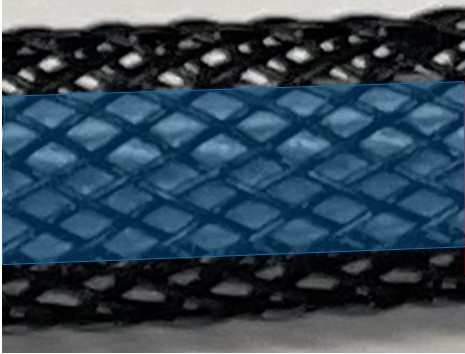
\includegraphics[scale=0.4]{image/hikaku_MPA_1.jpg}
    \subcaption{変化前}
    \label{fig:MPA_1}
  \end{minipage}
  %
  \begin{minipage}{0.49\hsize}
    \centering
    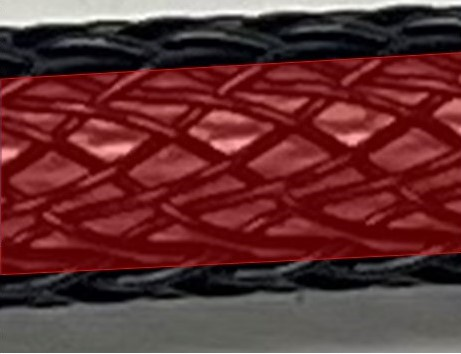
\includegraphics[scale=0.4]{image/hikaku_MPA_2.jpg}
    \subcaption{変化後}
    \label{fig:MPA_2}
  \end{minipage}
  %
  \caption{細径MPAの熱可塑変化の様子}
  \label{fig:MPA_henka}
\end{figure}
%
\begin{figure}[ht]
  \centering
  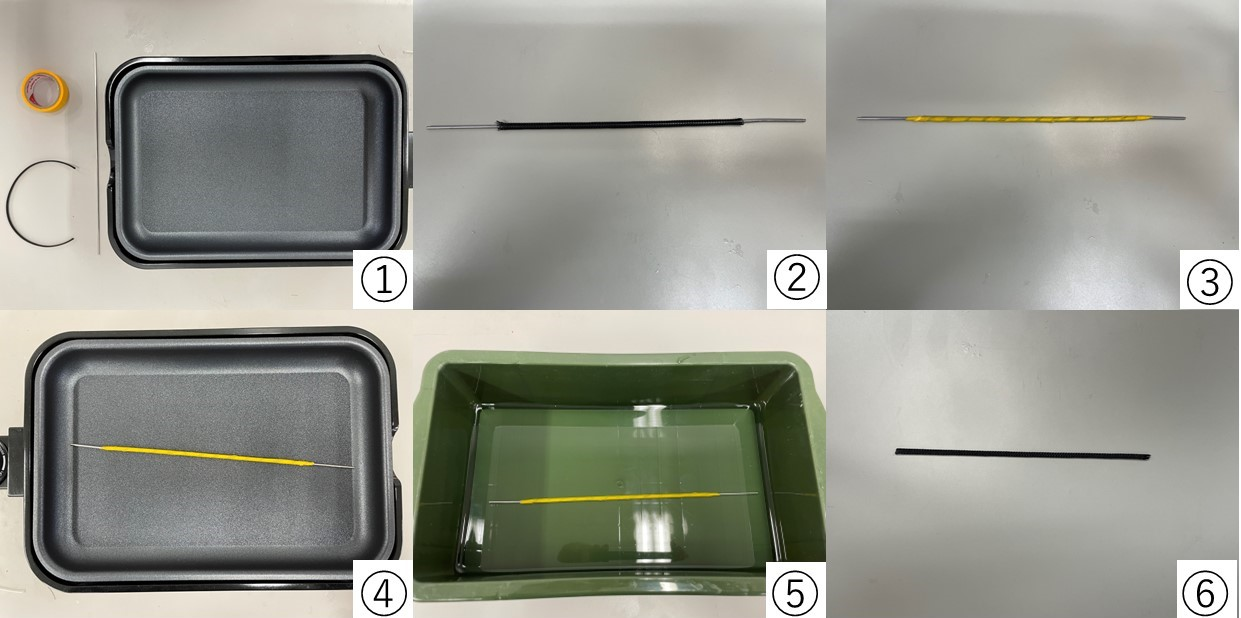
\includegraphics[scale=0.4]{image/messhu_tejyun.jpg}
  \caption{熱可塑変化の手順}
  \label{fig:messhu_method}
\end{figure}
%
%%%%%%%%%%%%%%%%%%%%%%%%%%%%%%%%%%%%%%%%%%%%%%%%%%%%%%%%%
\clearpage
\subsection{課題3:羽状角の変化に対する対応}
細径MPAを用いた羽状筋の動作の模式図を図\ref{fig:ujyoukin_moshiki}に示す.細径MPAが収縮すると,腱は赤い矢印の方向へ引っ張られる.
そして,細径MPAと腱とのなす角(羽状角)が変化することにより関節が回転する.
しかし,先行研究で作製された歩脚ロボット(図\ref{fig:ujyoukin_kako})では細径MPA端部の部品の角度が固定されていた.
それが原因で,細径MPAが収縮する際に端部部品と細径MPAが干渉してしまい腱を十分に引き込むことができなかった.
そこで本研究では細径MPAの収縮に応じて羽状角が変化する端部部品を開発した.開発した端部部品を図\ref{fig:tanbu_parts_new}\subref{fig:tanbu_parts}に示す.細径MPA端部の作製方法,手順を以下に示す.
\vspace{3mm}
\begin{enumerate}
  \item 図\ref{fig:tanbu_parts_new}\subref{fig:tanbu_parts}中\textcircled{\scriptsize 1},\textcircled{\scriptsize 2},\textcircled{\scriptsize 3}をSolidWorksを用いて設計する
  \item 光造形方式の3Dプリンターで印刷する.
  \item 図\ref{fig:tanbu_parts_new}\subref{fig:tanbu_parts}中の\textcircled{\scriptsize 3}の赤枠部分を図\ref{fig:tanbu_parts_new}\subref{fig:tanbu_parts}中\textcircled{\scriptsize 1},\textcircled{\scriptsize 2}で挟み込む
  \item 図\ref{fig:tanbu_parts_new}\subref{fig:tanbu_parts}中\textcircled{\scriptsize 1},\textcircled{\scriptsize 2}の隙間が空いていないことを確認したら完成
\end{enumerate}
次にこの部品の主な動作について説明する.先ほど説明した部品を組み立てた後(図\ref{fig:tanbu_parts_new}\subref{fig:tanbu_parts}中\textcircled{\scriptsize 3})の模式図を図\ref{fig:tanbu_parts_new}\subref{fig:tanbu_moshikizu}に示す.
図\ref{fig:tanbu_parts_new}\subref{fig:tanbu_moshikizu}中の赤斜線部の穴に回転軸が左右からはまる構造になっている.
これにより,端部部品に1自由度を持たせることができた.さらに,細径MPAの収縮に合わせて羽状角が変化することができ,端部部品と細径MPAが干渉しないことが確認することができた.
%%%%%%%%%%%%%%%%%%%%%%%%%%%%%%%%%%%%%%%%%%%%%%%%%%%%%%%%%
%
\begin{figure}[ht]
  \centering
  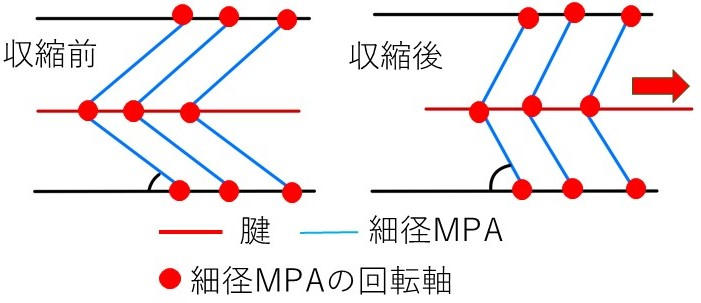
\includegraphics[scale=0.5]{image/ujyoukin.jpg}
  \caption{羽状筋の動作の模式図}
  \label{fig:ujyoukin_moshiki}
\end{figure}
%
\begin{figure}[ht]
  %
  \begin{minipage}{0.49\hsize}
    \centering  
    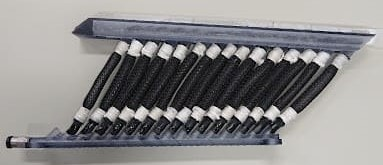
\includegraphics[scale=0.6]{image/yobi_syuseki.JPG}
    \subcaption{旧型羽状筋}
    \label{fig:ujyoukin_real_kako}
  \end{minipage}
  %
  \begin{minipage}{0.49\hsize}
    \centering
    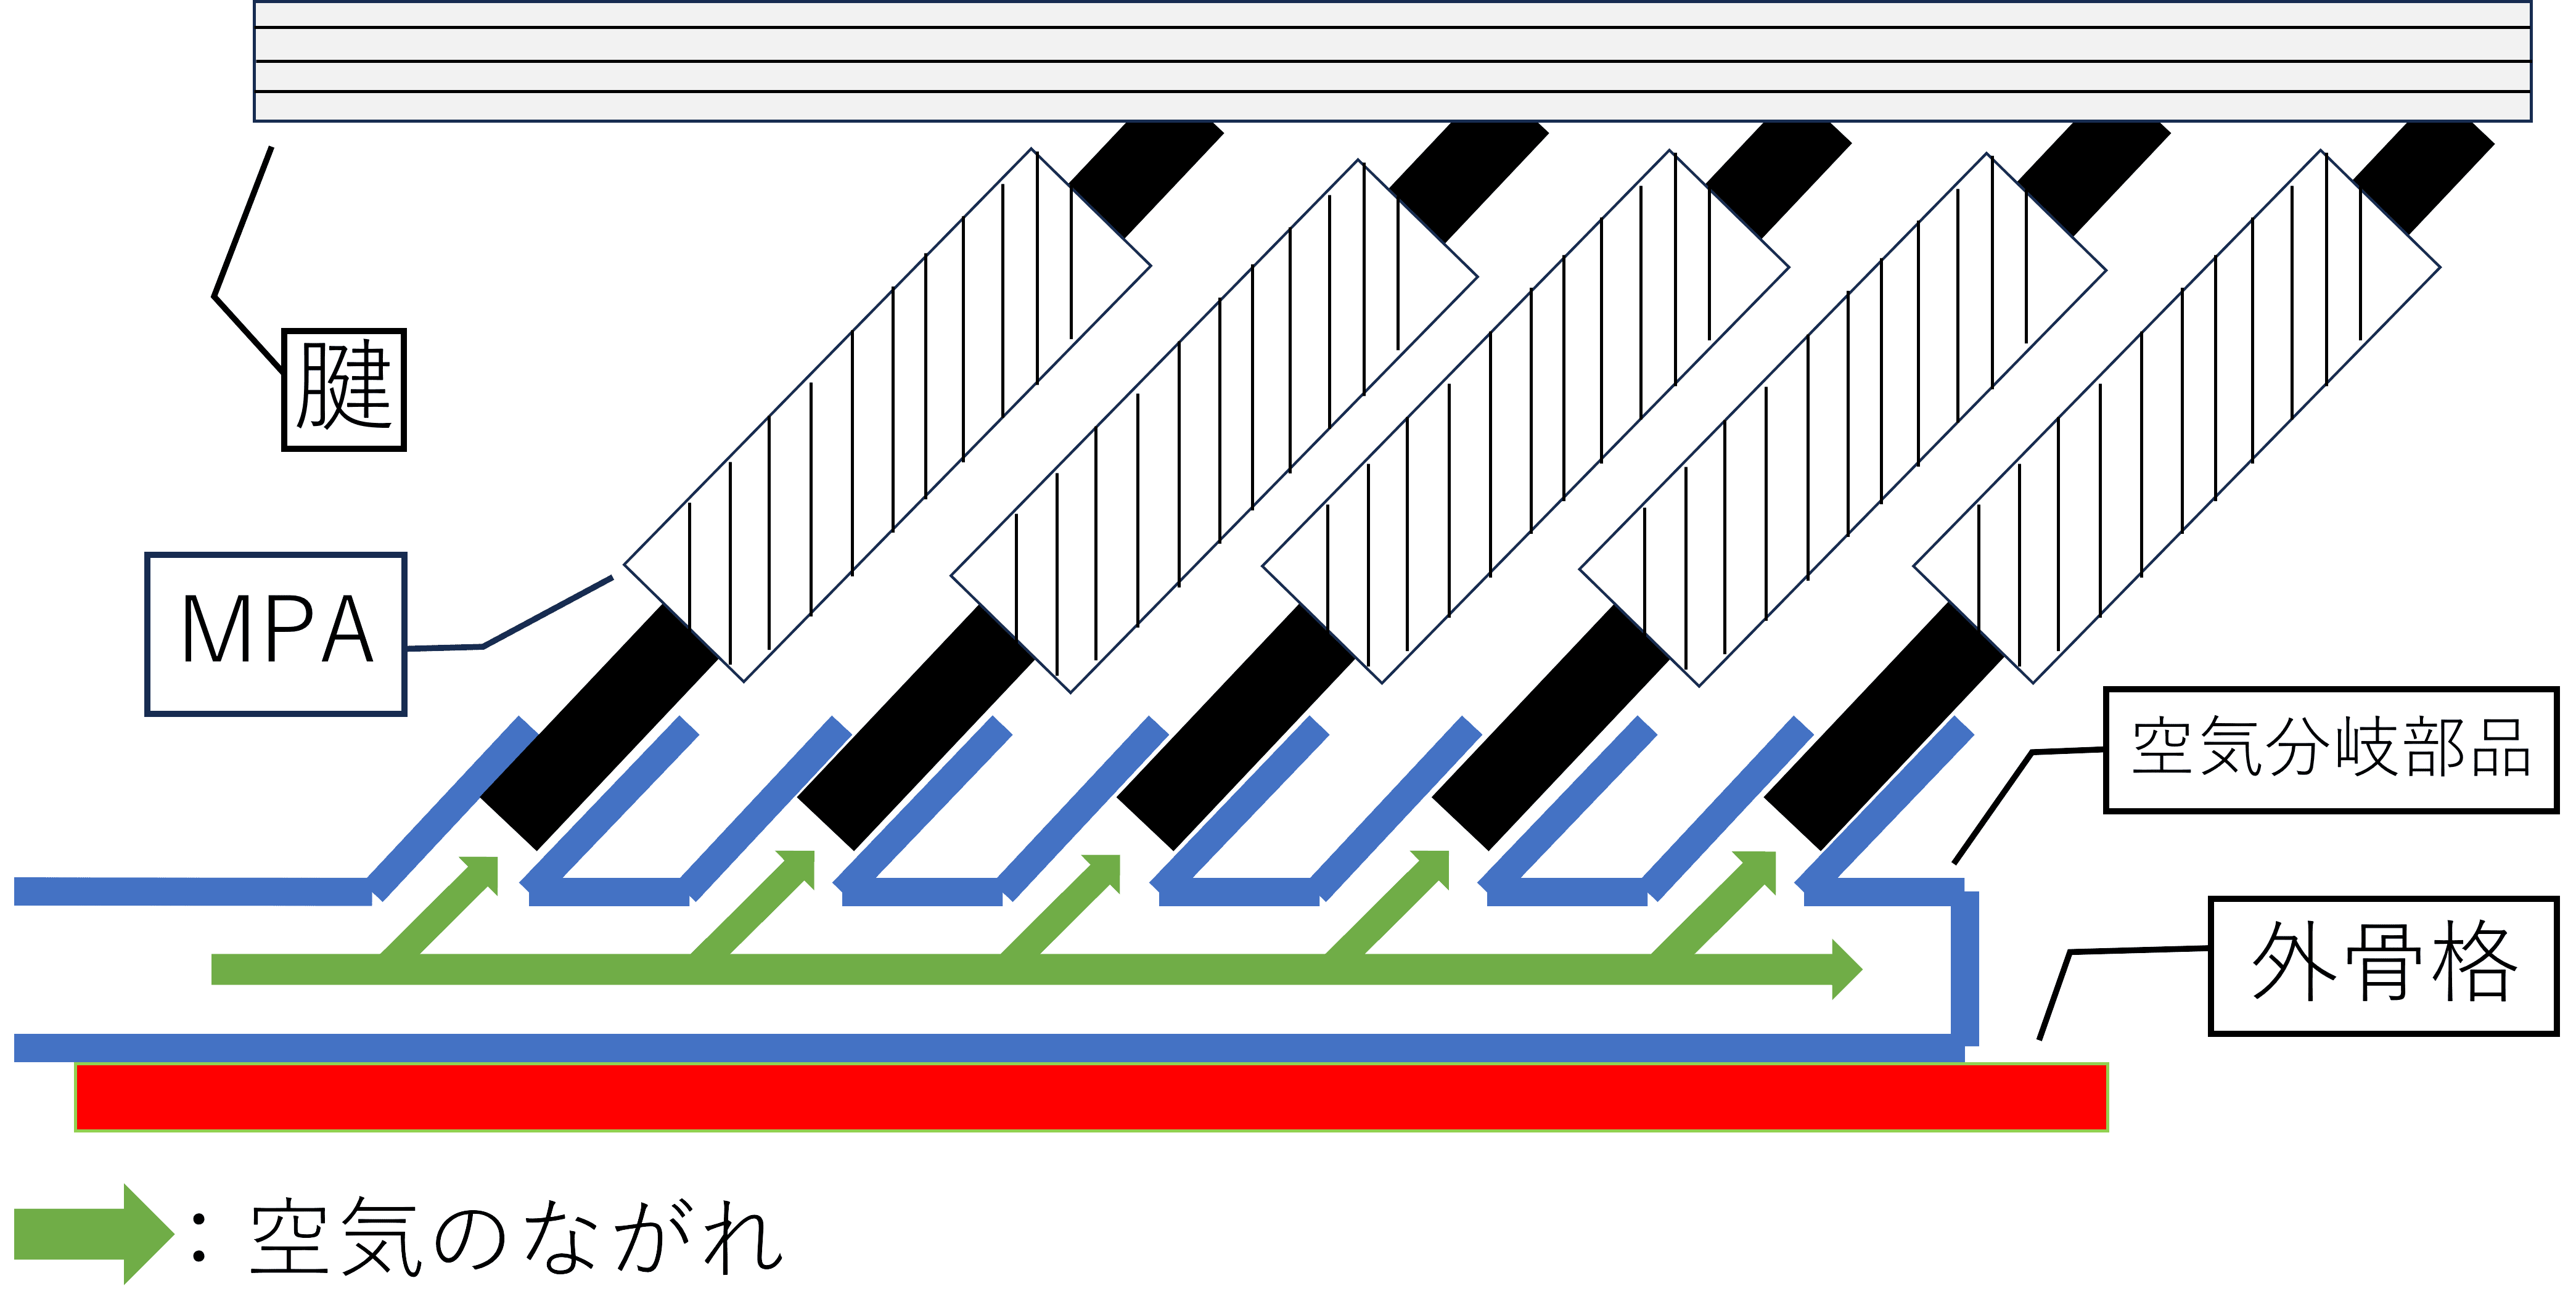
\includegraphics[scale=0.04]{image/air_moshiki.png}
    \subcaption{模式図}
    \label{fig:ujyoukin_moshiki_kako}
  \end{minipage}
  %
  \caption{先行研究で開発された羽状筋}
  \label{fig:ujyoukin_kako}
\end{figure}
%
\begin{figure}[ht]
  %
  \begin{minipage}{0.59\hsize}
    \centering  
    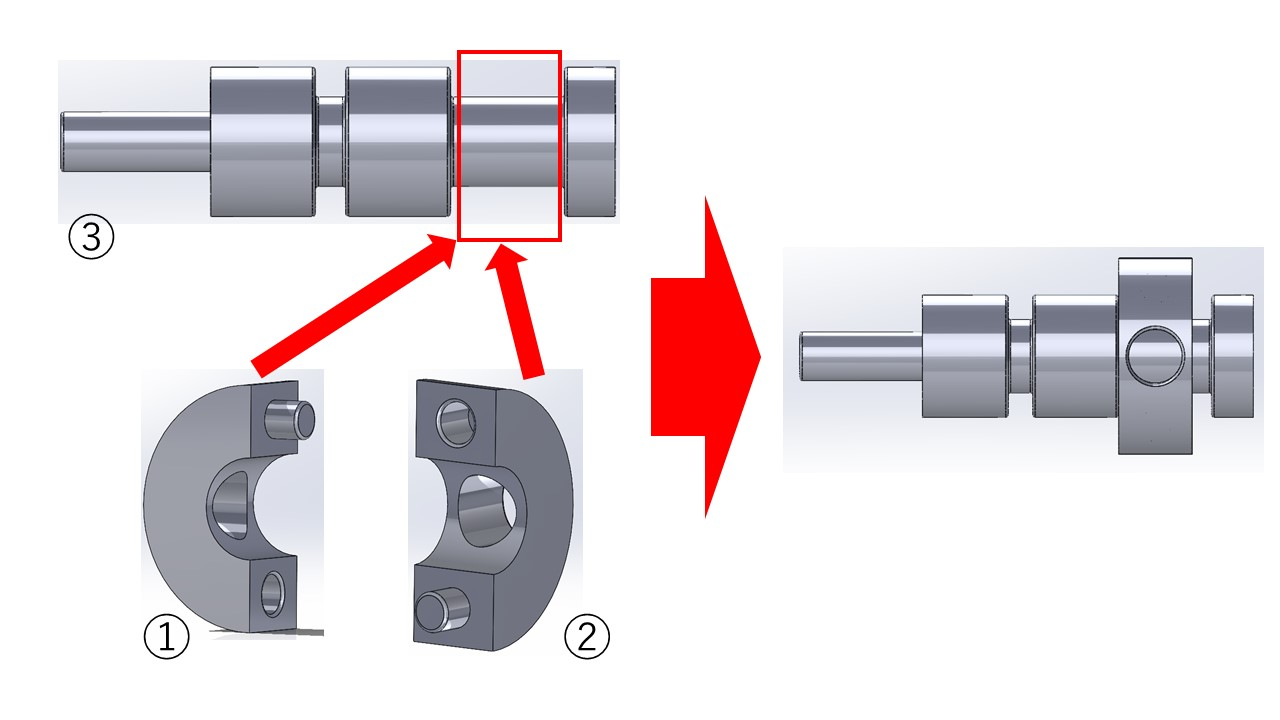
\includegraphics[scale=0.27]{image/tanbu_parts.jpg}
    \subcaption{組み立て方法}
    \label{fig:tanbu_parts}
  \end{minipage}
  %
  \begin{minipage}{0.39\hsize}
    \centering
    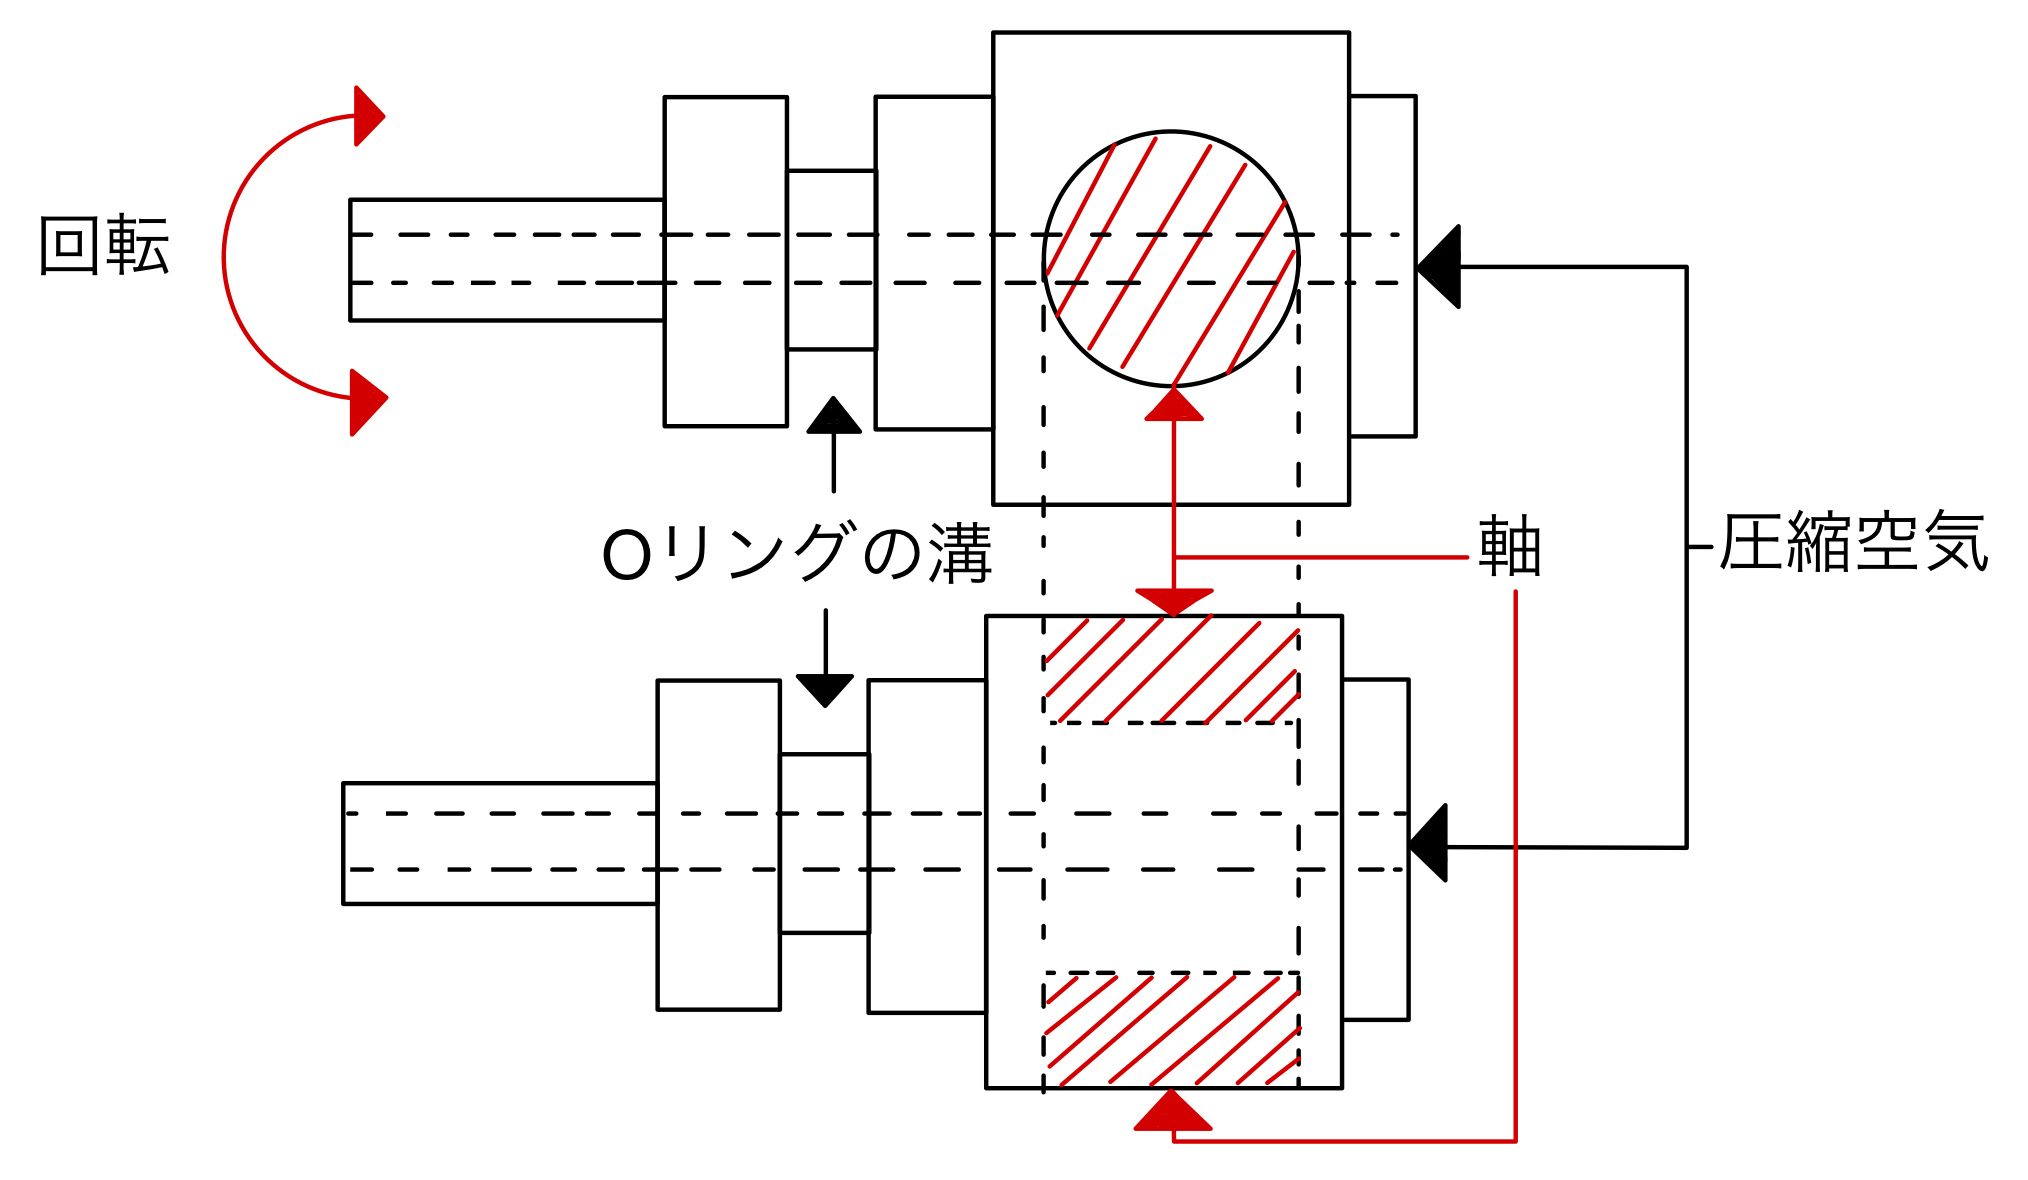
\includegraphics[scale=0.085]{image/MPA_irast.jpg}
    \subcaption{模式図}
    \label{fig:tanbu_moshikizu}
  \end{minipage}
  %
  \caption{先行研究で開発された羽状筋}
  \label{fig:tanbu_parts_new}
\end{figure}
%%%%%%%%%%%%%%%%%%%%%%%%%%%%%%%%%%%%%%%%%%%%%%%%%%%%%%%%%
\subsection{改良型細径羽状筋}
本研究で開発した改良型細径空圧羽状筋を図\ref{fig:ujyoukin_new}に示す.前述した先行研究の課題1,2,3の解決方法を取り入れて羽状筋を開発した.
図\ref{fig:ujyoukin_new}中の腱は柔軟な素材であるTPUを用いてFDM方式3Dプリンターで,細径MPA固定部品は光造形方式の3Dプリンターでそれぞれ作成した.
外骨格内部に配置可能な最大の長さの改良型細径空圧羽状筋を各節で作製した.その結果,解禁と平均で細径MPAの数が同じでそれぞれ1列ずつの構成となった.
長節では腱の上下ともに7本ずつ,腕節では腱の上側が5本で下側が4本,前節では腱の上下ともに4本ずつで羽状筋を作製した.
また,3章2節で述べた数理モデルのを用いた可動域の計算と作製の容易さから,細径MPAの長さは全て同じになるように作製した.
%%%%%%%%%%%%%%%%%%%%%%%%%%%%%%%%%%%%%%%%%%%%%%%%%%%%%%%%%
%
\begin{figure}[ht]
  \centering
  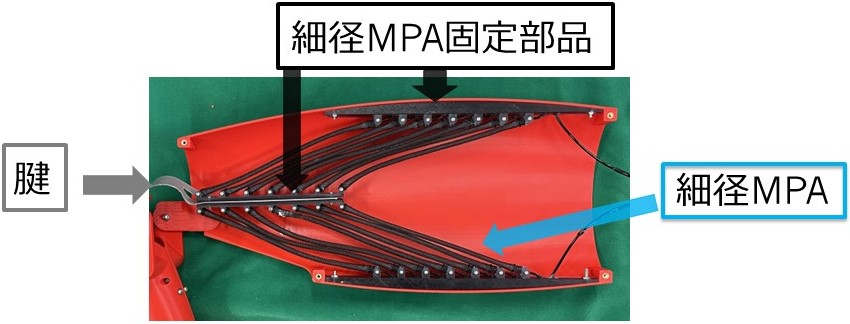
\includegraphics[scale=0.7]{image/uyjoukin_new.jpg}
  \caption{改良型細径空圧羽状筋}
  \label{fig:ujyoukin_new}
\end{figure}
%
%%%%%%%%%%%%%%%%%%%%%%%%%%%%%%%%%%%%%%%%%%%%%%%%%%%%%%%%%
%本研究で用いる3 mmの細径MPAの作製方法について説明する.
%構造は2.1節で述べた従来のMPAと同様,シリコンゴムチューブをナイロン繊維メッシュで覆ったシンプルなもので,0.4~0.6 MPaで駆動し収縮率は約20 %である.
%おおまかな作製手順を図\ref{fig:shingata_sakuseihouhou}に示す.
%端部の締結方法はOリングを用いる方法を採用した.
%図中\textcircled{\scriptsize 1}に示した物品が作製に必要なもので左から以下の通りである.
%
%\begin{itemize}
%  \item PPX(瞬間接着剤) メーカー:セメダイン 品番:CA-522
%  \item シリコンゴムチューブ 2×3(内径×外径) メーカー:タイガースポリマー 品番:SR1554
%  \item ポリウレタンチューブ 2×1.2(外径×内径) メーカー:PISCO 品番:UB0212-20-B
% \item 編組チューブ 1×5(最小径×最大径) メーカー:モノタロウ 品番:-
%  \item 光造形で作製した細径MPA端部部品
%\end{itemize}
%
%以下,作成手順である.
%
%\begin{enumerate}
%  \item まず初めにシリコンゴムチューブを任意の長さで切り,ナイロンメッシュをシリコンゴムチューブより5 cm程長く切る
%  \item シリコンゴムチューブの両端をそれぞれ光造形の部品の溝に差し込み,部品とシリコンゴムチューブの間に接着剤を塗布する(図中\textcircled{\scriptsize 2})
%  \item 接着剤が十分に乾いたら編組チューブを被せる(図中\textcircled{\scriptsize 3})
%  \item ナイロンメッシュを押さえつけ,かつ光造形のOリング固定溝にはまるようにOリングを配置する.固定する際にナイロンメッシュが緩まないようにOリングを固定する(図中\textcircled{\scriptsize 4})
%  \item 締結した部分に接着剤を塗布し,緩まないようにする
%  \item 接着剤が十分に乾いたら余分なナイロンメッシュを切り取る(図中\textcircled{\scriptsize 5})
%  \item ポリウレタンチューブを光造形の部品に差し込み,部品とポリウレタンチューブの間に接着剤を塗布し乾燥させて完成
%\end{enumerate}
%%%%%%%%%%%%%%%%%%%%%%%%%%%%%%%%%%%%%%%%%%%%%%%%%%%%%%%%%
%\begin{figure}
%  \centering
%  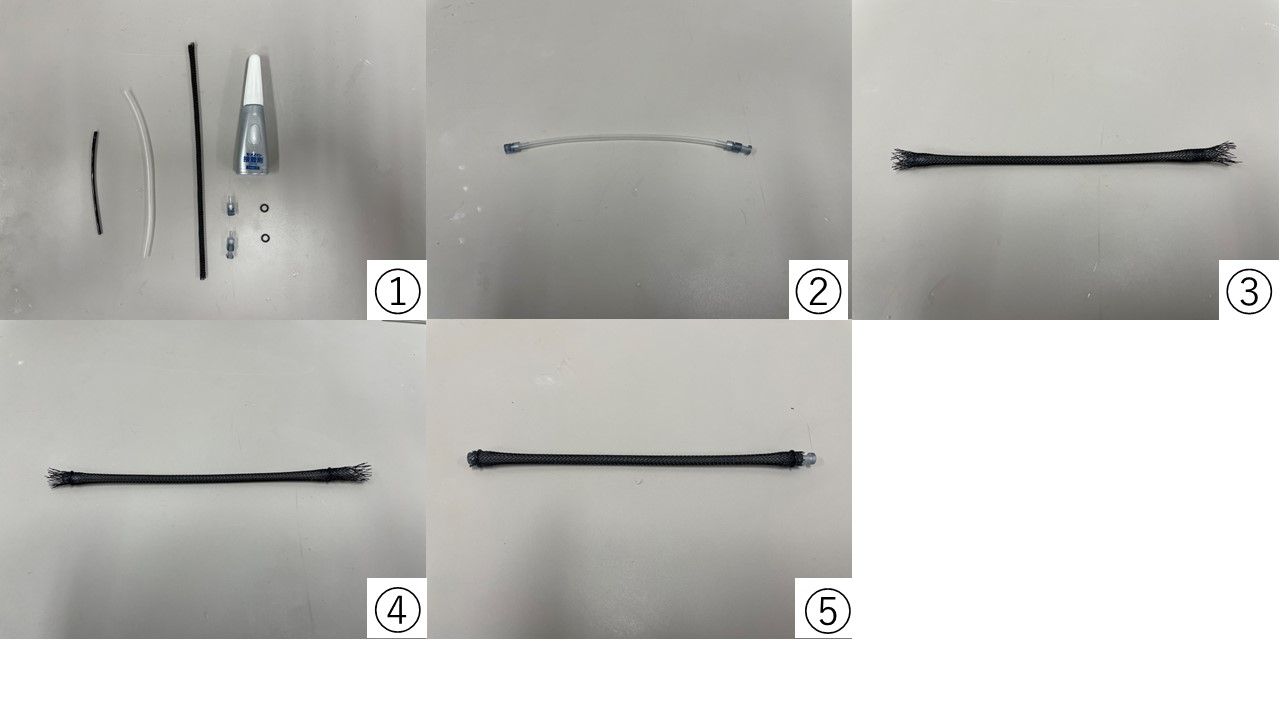
\includegraphics[scale=0.4]{image/sakusei.jpg}
%  \caption{改良型細径MPAの作製方法}
% \label{fig:shingata_sakuseihouhou}
%\end{figure}
%%%%%%%%%%%%%%%%%%%%%%%%%%%%%%%%%%%%%%%%%%%%%%%%%%%%%%%%%

